% !TeX root = paper.tex
% !TeX spellcheck = en_US
% !TeX program = pdflatex
% !TeX encoding = UTF-8

\documentclass[a4paper, 11pt]{scrartcl}

\usepackage[utf8]{inputenc}
\usepackage[T1]{fontenc}
\usepackage{graphicx}

\usepackage[hidelinks]{hyperref}
\usepackage[acronym]{glossaries}
\usepackage[shorthands=off, english]{babel}
\usepackage[autostyle]{csquotes}
\usepackage{amsmath,amssymb,amsfonts}

\pdfcompresslevel=0

\title{Title} % TODO adapt title
\subtitle{Group \#} % TODO change group number
\author{Student A.\\\href{mailto:studenta@hochschule-burgenland.at}{studenta@hochschule-burgenland.at} \and Student B.\\\href{mailto:studentb@hochschule-burgenland.at}{studentb@hochschule-burgenland.at} } % TODO change authors


%%%%%%%%%%%%%%%%%%%%%%%%%%%%%%%%%%%%%%%%%%%%%%%%%%%%%%%%%%%%%
%% DOCUMENT
%%%%%%%%%%%%%%%%%%%%%%%%%%%%%%%%%%%%%%%%%%%%%%%%%%%%%%%%%%%%%
\begin{document}
\maketitle

\begin{abstract}
Tick the boxes for the level your implementation achieves: 

\begin{itemize}
    \item[$\boxtimes$] Minimal
    \item[$\square$] Advanced
    \item[$\square$] Expert
\end{itemize}
\end{abstract}

\section{Work Distribution}

Provide a short paragraph describing the contribution of each team member. Clearly state which tasks and responsibilities were carried out by whom during the project (e.g., agent implementation, architecture design, testing, documentation).

\section{Problem Statement}

Describe your detection system.

\begin{figure}[ht]
    \centering
    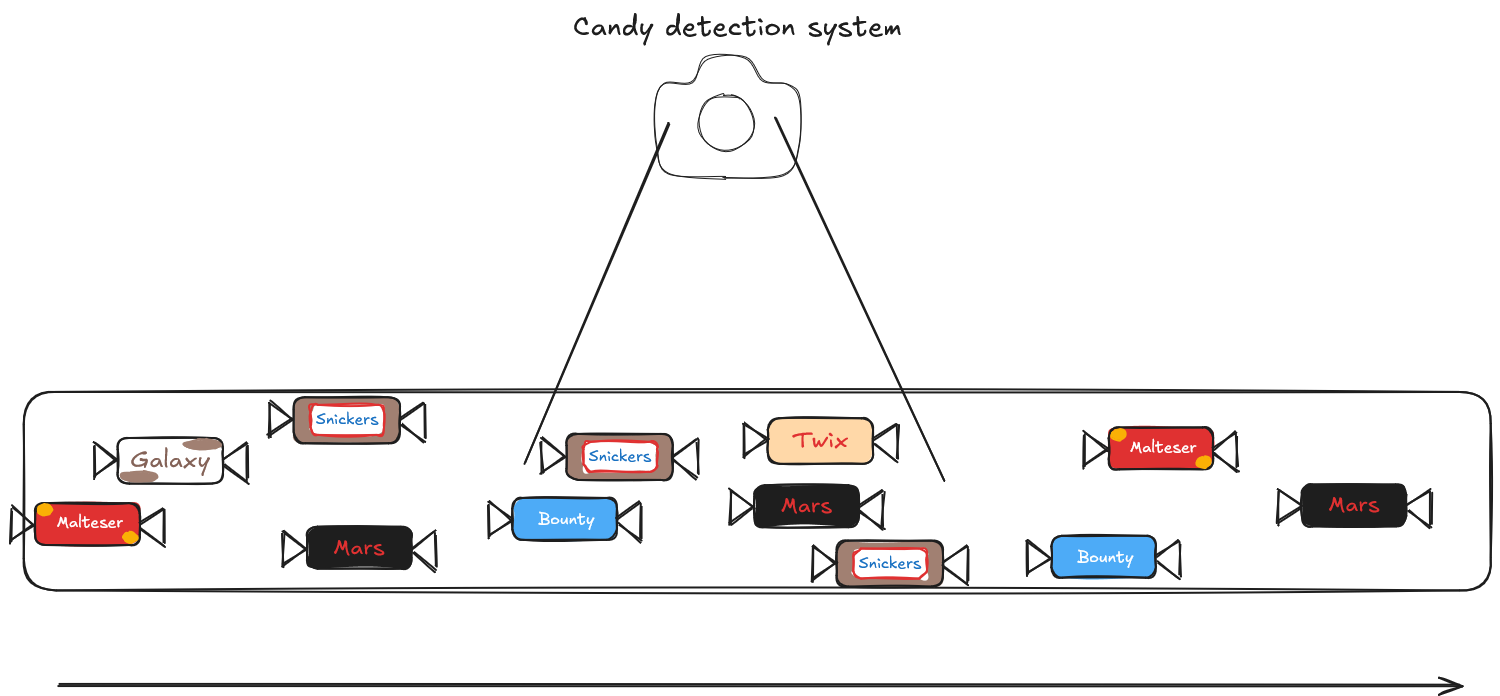
\includegraphics[width=0.8\linewidth]{figures/candy_detection_system}
    \caption{Candy detection system}
    \label{fig:candy_detection_system}
\end{figure}

\section{Pre-Processing}

\section{Transfer-Learning}

\section{Evaluation}

%--------Delete------------------
\section{Ease of Use - Delete in your final version!}

\subsection{Abbreviations and Acronyms}\label{AA}
Define abbreviations and acronyms the first time they are used in the text, 
even after they have been defined in the abstract. Do not use 
abbreviations in the title or heads unless they are unavoidable.

\subsection{Units}
\begin{itemize}
\item Use either SI (MKS) or CGS as primary units. (SI units are encouraged.) English units may be used as secondary units (in parentheses). An exception would be the use of English units as identifiers in trade, such as ``3.5-inch disk drive''. 
\item Avoid combining SI and CGS units, such as current in amperes and magnetic field in oersteds. This often leads to confusion because equations do not balance dimensionally. If you must use mixed units, clearly state the units for each quantity that you use in an equation.
\item Do not mix complete spellings and abbreviations of units: ``Wb/m\textsuperscript{2}'' or ``webers per square meter'', not ``webers/m\textsuperscript{2}''. Spell out units when they appear in text: ``. . . a few henries'', not ``. . . a few H''.
\item Use a zero before decimal points: ``0.25'', not ``.25''. Use ``cm\textsuperscript{3}'', not ``cc''.)
\end{itemize}

\subsection{Equations}
Number equations consecutively. To make your equations more compact, you may use the solidus (~/~), the exp function, or appropriate exponents. Italicize Roman symbols for quantities and variables, but not Greek symbols. Use a long dash rather than a hyphen for a minus sign. Punctuate equations with commas or periods when they are part of a sentence, as in:
\begin{equation}
a+b=\gamma\label{eq}
\end{equation}

Be sure that the symbols in your equation have been defined before or immediately following the equation. Use ``\eqref{eq}'', not ``Eq.~\eqref{eq}'' or ``equation \eqref{eq}'', except at the beginning of a sentence: ``Equation \eqref{eq} is . . .''

\subsection{Figures and Tables}
\paragraph{Positioning Figures and Tables} Place figures and tables at the top and bottom of columns. Avoid placing them in the middle of columns. Large figures and tables may span across both columns. Figure captions should be below the figures; table heads should appear above the tables. Insert figures and tables after they are cited in the text. Use the abbreviation ``Fig.~\ref{fig:candy_detection_system}'', even at the beginning of a sentence.

\begin{table}[htbp]
\caption{Table Type Styles}
\begin{center}
\begin{tabular}{|c|c|c|c|}
\hline
\textbf{Table}&\multicolumn{3}{|c|}{\textbf{Table Column Head}} \\
\cline{2-4} 
\textbf{Head} & \textbf{\textit{Table column subhead}}& \textbf{\textit{Subhead}}& \textbf{\textit{Subhead}} \\
\hline
copy& More table copy$^{\mathrm{a}}$& &  \\
\hline
\multicolumn{4}{l}{$^{\mathrm{a}}$Sample of a Table footnote.}
\end{tabular}
\label{tab1}
\end{center}
\end{table}

\subsection{References}

Please number citations consecutively within brackets \cite{dunkels2004contiki}. The sentence punctuation follows the bracket \cite{dunkels2004contiki}. Refer simply to the reference number, as in \cite{dunkels2004contiki}---do not use ``Ref. \cite{dunkels2004contiki}'' or ``reference \cite{dunkels2004contiki}'' except at the beginning of a sentence: ``Reference \cite{dunkels2004contiki} was the first $\ldots$''

\bibliographystyle{ieeetr}
\bibliography{references}

\end{document}
